\section{test}%
\label{sec:test}
To make Further observation with a laser, you have to attitude it first. 
First thing to do is to calibrate the current to achieve a population inversion. 
For makeing the laser light visible the laser is pointed to a buisnesscardholder
which is filmed by a ccd sensor.
\begin{figure}[h]
		\centering
		\includegraphics[width=0.8\linewidth]{./build/emissionconstruction.pdf}
		\caption{Buisness Card Plot should be here}
		\label{fig:aufbau}
\end{figure}
To achieve the minimal current to laser by induce emission, aternately the head
knob and side knob position is optimized.
Everythime stimulated emission is produce, current is shutting down power a
little bit. 
So that the last visible induce emission is the minimal laser current. 
A Note for stimulated emission is that the light cone from induced emission is
much brighter and more homegenous than by spontanious Emission.
One Example for induce \ref{fig:induce} and spontanious \ref{fig:spontanious} light cone is shown in picture \ref{fig:emission}.
\begin{figure}[h]
		\centering
		\begin{subfigure}[b]{0.45\textwidth}
				\begin{center}
						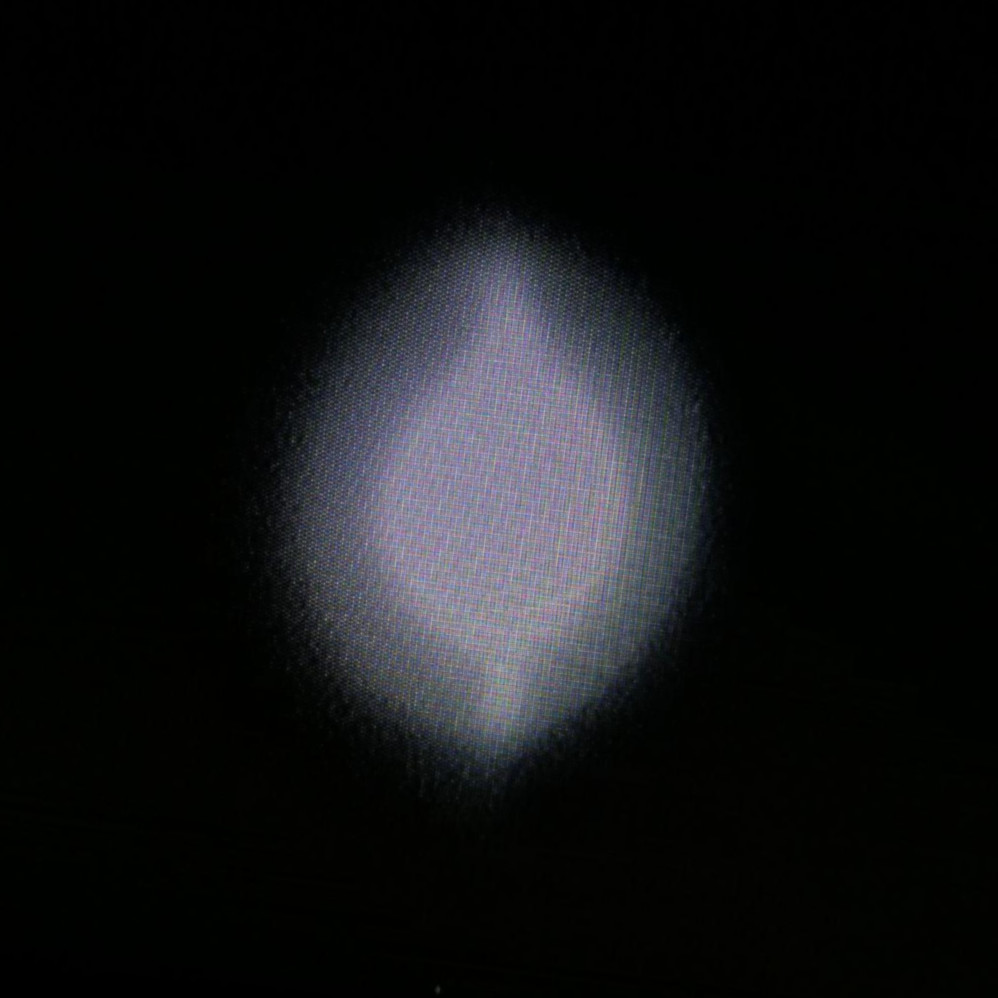
\includegraphics[width=0.9\linewidth]{./content/pictures/below_threshold.jpg}
						\caption{spontanious emission}
				\label{fig:spontanious}
				\end{center}
		\end{subfigure}
		\begin{subfigure}[b]{0.45\textwidth}
				\begin{center}
						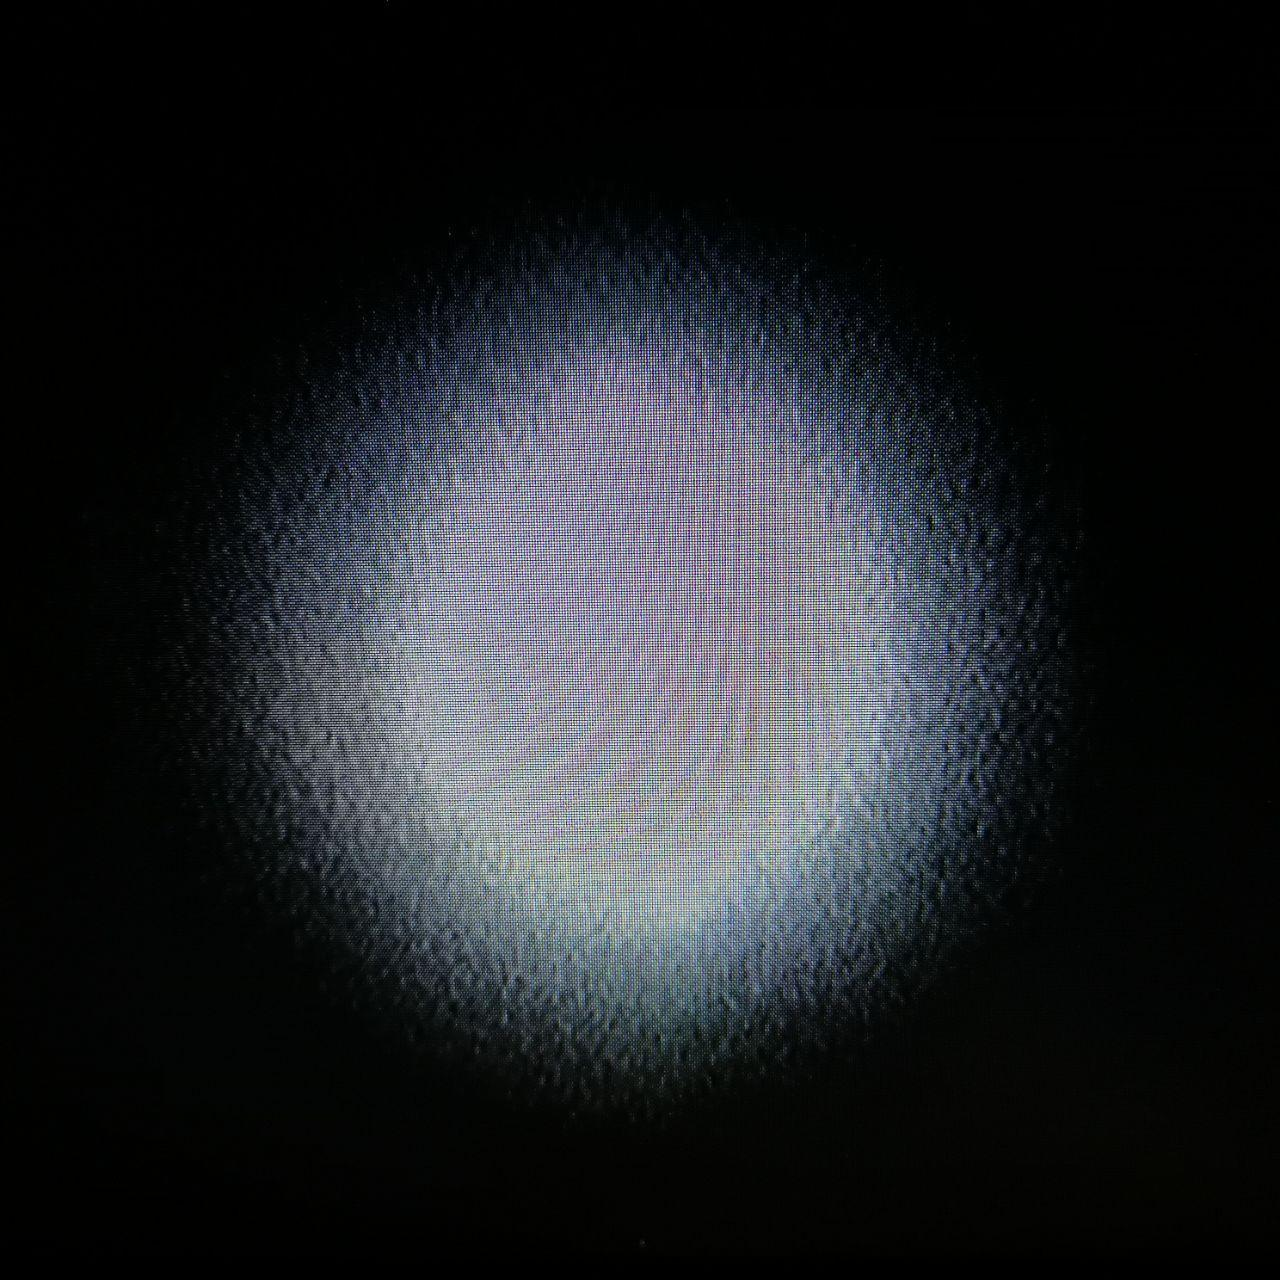
\includegraphics[width=0.9\linewidth]{./content/pictures/above_threshold.jpg}
						\caption{induce emission}
						\label{fig:induce}
				\end{center}
		\end{subfigure}
		\caption{threshold emission}
		\label{fig:emission}
\end{figure}
The meassured current for the minimal threshold is \SI{30}{\milli\ampere}.
By moving both knobs over full range, no flashes can be generated.


\subsection{Anregen Rubidium}%
\label{sub:anregen_rubidium}

To stimulated the rubidium Gas beam Angle has to pass the chamber so that no
light is ideal sprinkeld at the border of the chamber. 
In Figure \ref{fig:hole_emission} is shown how the measureing instrumente have to be
arrange to measure the light intensity.
\begin{figure}[h]
		\centering
		\includegraphics[width=0.8\linewidth]{build/rubidiumemission.pdf}
		\caption{}
		\label{fig:hole_emission}
\end{figure}
The Voltage of the photo diode is increased and shown on an oszilloskop. 
The side knob have to be calibrate to attain the right frequenz for stimulated
the gas. 
For reducing the contrast a gratting is put in the beam so that the beamangle
can be seen with help of a ccd Camera. 
Right frequenz is be found if in the Camera a small beam is visible. 
The middle beam of side knob variation should be choosen because it had the
srongest gain.
An example for ionizing Gas is shown in figure \ref{fig:ionized}.
\begin{figure}[h]
		\centering
		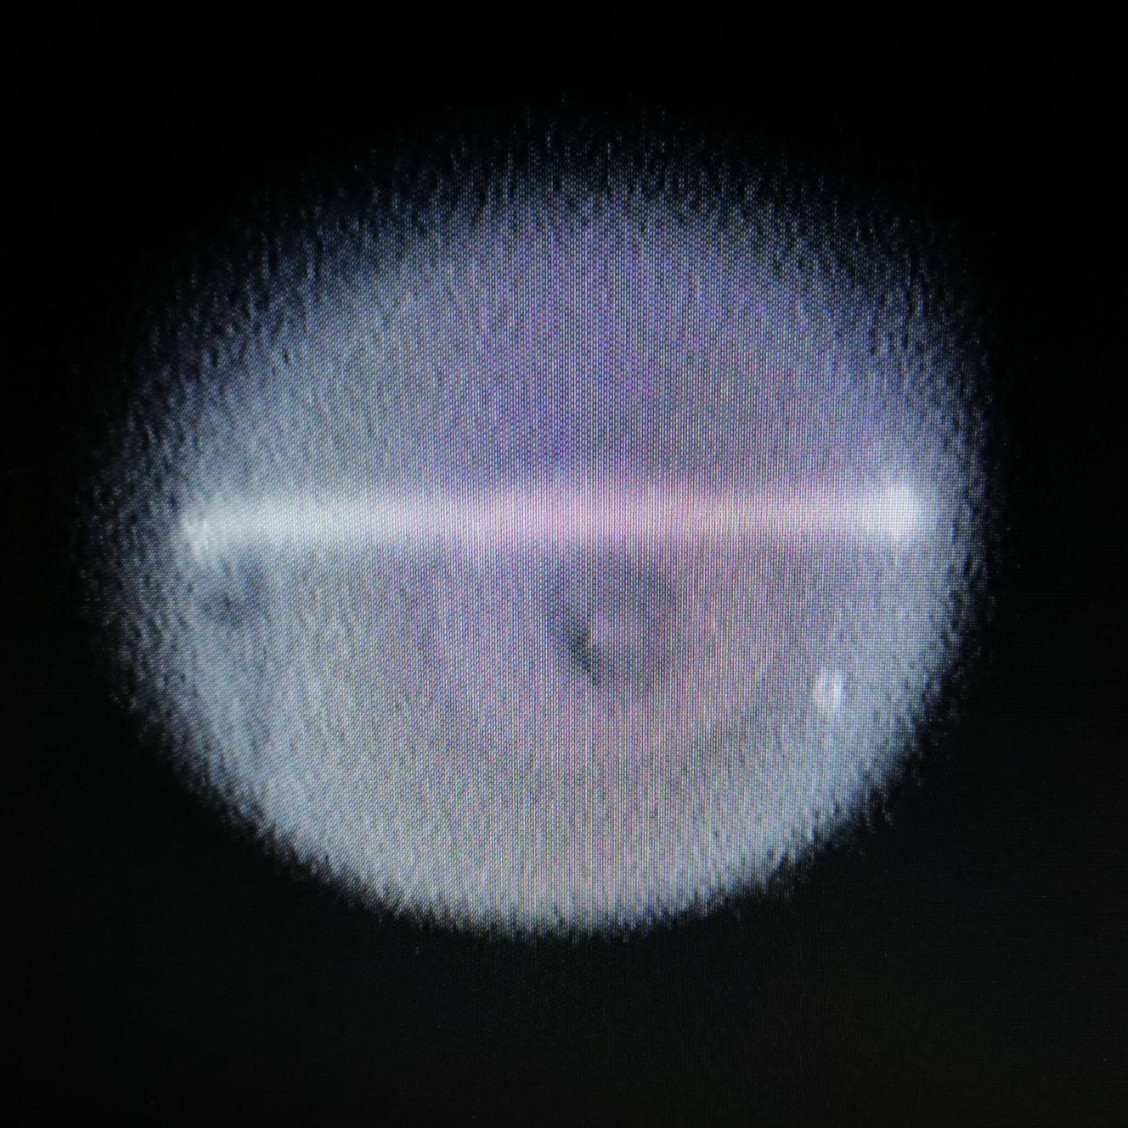
\includegraphics[width=0.4\linewidth]{./content/pictures/fluorescence.jpg}
		\caption{}
		\label{fig:ionized}
\end{figure}
Aim after the Robidium is stimulated is to meassure the absorption spektrum. 

\subsection{Absorbtion Spektrum}%
\label{sub:absorbtion_spektrum}

A absorption Spektrum is dependence from the frequence. 
To achieve a variation in frequence a pieco element is used. 
The piezo element is on the diffraction gratting to variated the length of the
external resonator. 
Varation of resonator length causes shifts in laser frequenz. 
Piezo element is powerd by a ramp generator which causes linear shifts in
resonator length in a defined time period.
When Photocurrent is meassured by a sensor dependence between energy niveaus can
be ploted.
\begin{figure}[h]
		\centering
		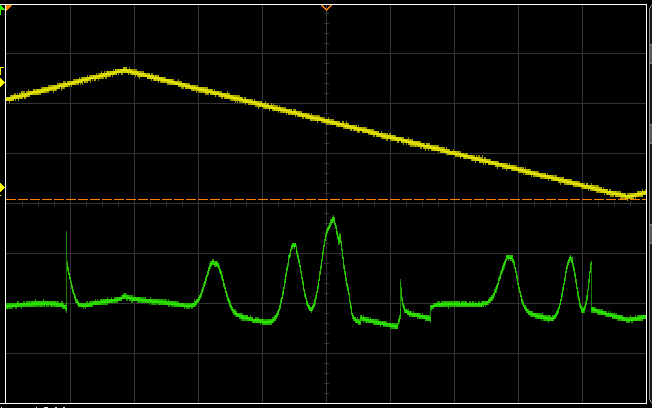
\includegraphics[width=0.8\linewidth]{./content/pictures/scope_136.png}
		\caption{}
		\label{fig:piezotest}
\end{figure}
In figure \ref{fig:piezotest} the yellow line shows the voltage at the Piezo
element which causes frequenz variation proportional to voltage.
The green line is photo stream. 
Hopes in the Photostream are horizontal modes caused by the Piezo element.
They are of no further interest.
To reduce mode hopping piezo modulation will be used. 
The response is the graphic below (figure \ref{fig:rectangular}).
\begin{figure}[h]
		\centering
		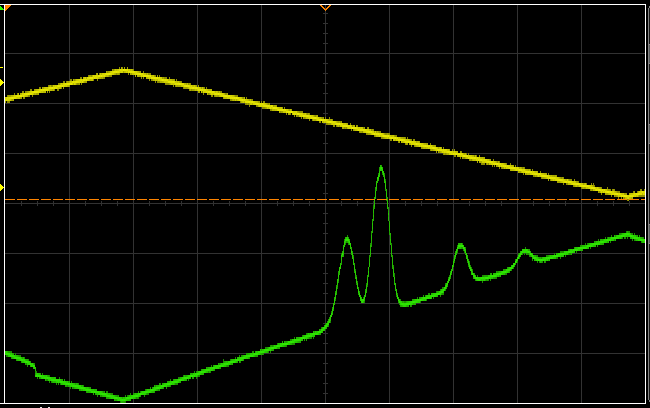
\includegraphics[width=0.8\linewidth]{./content/pictures/scope_138.png}
		\caption{}
		\label{fig:rectangular}
\end{figure}
The caracteristic Spektrum of a rubidium crystall is visible which the
absorption lines. 
In general the green line should be mirrored on the x-axis because resonance
reduce the Energy on the photonstream. 
For achieving a flat sprectrum which is not depended of the piezo voltage some
modifikation are necessary.

\subsection{The perfect spectrum}%
\label{sub:the_perfect_spectrum}

For modulation of the pure laserbeam and this which pass the medium one, beam
will be splited in two parts. 
A semipermeable mirrow will be set in the beam path for the medium. 
Light which reflected before the medium will be measured by a second Photomultiplier.
Now beam modulation with a part which not passes and a part which passes the
medium can be done. 
The absorption spectrum without piezo movement effect is shown in figure
\ref{fig:modulation}.
\begin{figure}[h]
		\centering
		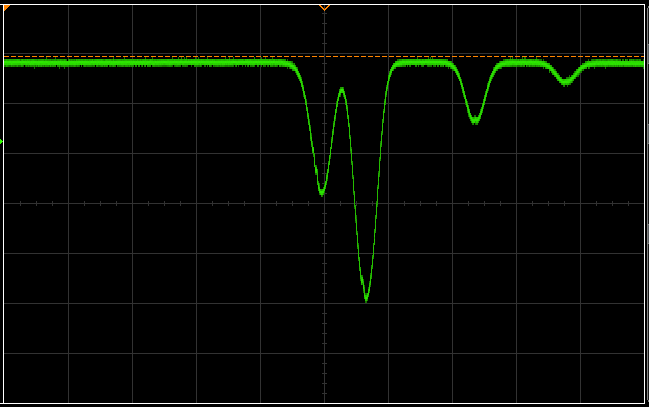
\includegraphics[width=0.8\linewidth]{./content/pictures/scope_140.png}
		\caption{}
		\label{fig:modulation}
\end{figure}
There are the different energielevels (85\sfrac{a}{b}, 87\sfrac{a}{b}) are
shown.
Know the laser is alignet and ready for further experiment.
